\documentclass[11 pt, titlepage]{article}
\usepackage[english]{babel}
\usepackage[utf8]{inputenc}
\usepackage[text={165mm,215mm}]{geometry}  %Størrelse på effektiv papir
\usepackage{abstract}
\usepackage{amsmath}

%Physics packages
\usepackage{physics}
\usepackage{tikz}
\usepackage{siunitx}
\usepackage{xfrac}

%Appendix
\usepackage[title, titletoc]{appendix}

%Figure packages
\usepackage{graphicx}
\usepackage{wrapfig}
\usepackage[font={small}, labelsep = period, labelfont=bf]{caption}
\usepackage{subcaption}
\usepackage{setspace}

%Linjeafstande
\setlength{\parindent}{0em}
\setlength{\parskip}{0em}
\linespread{1.15}

%Litteraturliste og fodnoter
\usepackage[autostyle]{csquotes}
\usepackage[bibstyle=numeric, sorting=none, citestyle=numeric,backend=biber,abbreviate=true, block=none]{biblatex}
\setlength\bibitemsep{\baselineskip}
\bibliography{references.bib}
\addbibresource{references.bib}
\renewcommand{\intitlepunct}{ }
\renewcommand*{\subtitlepunct}{ - }
\usepackage[marginal,bottom]{footmisc}

% Frontpage text
\title{\vspace{2.7 cm}\\
\textbf{\LARGE{A Shot in the Dark: Finding Heavily Obscured Galaxies in Multi-Wavelength Surveys}} 
\\
\vspace{2 cm}
\Large{Bachelor Thesis}
\\
\vspace{1 cm}
\large{Supervised by Iary Davidzon,\\ Francesco Maria Valentino \\ and Johan Peter Uldall Fynbo }}
\author{\vspace{1 cm} \\ Kimi Cardoso Kreilgaard}
\date{Submission Date \\ 16.06.2021}

% Front page background
\usepackage{eso-pic}
\newcommand\BackgroundPic{%
\put(0,0){%
\parbox[b][\paperheight]{\paperwidth}{%
\vfill
\centering

\includegraphics[width=\paperwidth,height=\paperheight]{ku-front.pdf}%
\vfill
}}}

% Table of contents and sections
\usepackage{tocloft}
\renewcommand{\cftsecleader}{\cftdotfill{\cftdotsep}}

%-------------------------------------------------------------------------------
\begin{document}

% Make frontpage
\AddToShipoutPicture*{\BackgroundPic} 
\maketitle

% Acknowledgements and Abstract 
\pagenumbering{roman} %romerske sidetal
\renewcommand{\abstractname}{Acknowledgements}
\begin{abstract}
\thispagestyle{plain}
\pagenumbering{roman}
\setcounter{page}{1}
First and foremost, I wish to express my sincere gratitude to my main supervisors Iary Davidzon and Franscesco M. Valentino for their engagement and exceptional guidance during this project. I would like to give Iary a special thanks for his creativity and his patience with me during this project, and Fransesco, I thank, for his keen eye to detail. Finally, I would also like to thank Linea Hedemark for her great spirits and support during the COVID-19 lockdown where our thesis workdays proved invaluable for my productivity.
\end{abstract}
\pagebreak \clearpage

\renewcommand{\abstractname}{Abstract}
\addcontentsline{toc}{section}{Abstract}
\begin{abstract}
\thispagestyle{plain}
\pagenumbering{roman}
\setcounter{page}{2}
Recent work revealed a significant population of "hidden galaxies" in the early universe (redshift $z>3$), which systematically escaped optical and near IR telescope imaging due to high dust content. These peculiar "NIR-dropout galaxies" can now be identified in state-of-the-art infrared surveys, where the impact of dust is less strong.
This project proposes a semi-automated method for the identication of the most reliable candidates of "NIR-dropout galaxies". The technique takes advantage of unsupervised and semi-supervised machine learning to classify galaxies. In particular, we use t-distributed Stochastic Neighbour Embedding (t-SNE) for dimensionality reduction on unlabeled data, consisting of cutouts of telescope images in various bands. With information from the COSMOS catalogue we construct a combined model of the telescope image. Subtracting the model from the the scientific image we produce a residual map that is used for the detection of the objects constituting our sample. Through visual inspection of the residual image, a sample of respectively promising and unfit candidates is labelled to allow for semi-supervised classification of galaxies according to the vote of k neighbours. With this method we are able to classify $\sim300$ robust candidates from the entire sample of $\sim3000$ galaxies, thus reducing the sample to be visually insepcted by a factor of 10. This method will allow identification and classification of distant, optically faint galaxies among the millions of object that will be detected in next-generation surveys such as \textit{Euclid}. Upon confirmation of the candidates, this might lead to a challenge of our understanding of galaxy evolution and/or provide insight into the physical features of intrinsically faint, distant galaxies.

\textcolor{red}{Include link to github with code}
\textcolor{blue}{Upon confirmation of the candidates, through spectral analysis, this can lead to interesting further research. If the galaxies are intrinsically faint, and thus quiescent at a high redshift, they can challenge our understanding of galaxy evolution. If the galaxies are not intrinsically faint, they might prove to contain unprecedented amounts of dust and will complement our understanding of the physical features of faint galaxies.}

\end{abstract}

%Contentline
\newpage \clearpage
\thispagestyle{plain}
\pagenumbering{roman}
\setcounter{page}{3}
\tableofcontents

\newpage
%%%% DOCUMENT INPUT %%%%
\pagenumbering{arabic} %sidetal
\section{Introduction}
\begin{itemize}
    \item General properties of dusty galaxies and galaxy evolution - why is this interesting?
    \item Distant galaxies are studied through photometric analysis. A large catalogue theory is based on is the COSMOS 2015 (CLASSIC) catalogue.
    \item Problems with this catalogue and this method of studying galaxies. Recent work revealed "hidden galaxies" \cite{Wang_2019} and \cite{Alcalde_Pampliega_2019}. Also new catalogue FARMER that can be used for this.
    \item Suggests that a type of galaxies have been systematically overlooked due to their faintness. This project suggest a method automising the way we can identify these.
    \item Quick overview of how we will do it. Describe which sections to find it.
    \item What can we expect - anticipations
\end{itemize}


\section{Method}
\textcolor{blue}{Add an introduction to how the methods section is split into to parts adn what each will cover}.

\subsection{Producing a Residual Map and Performing Source Detection}
\textcolor{blue}{this section desperately needs some sub sub sections that can help structure the section}
A residual map is produced by modelling the light profiles of the detected sources and subtracting them from the scientific telescope image. Both the COSMOS 2015 and 2020 contain the information necessary to compute a residual map, but differ in their method of performing source extraction and thus also in their method of modelling sources. Since we are interested in objects that are visible in the IRAC bands and not visible in the NIR bands, we aim to produce a residual map of the IRAC image subtracting sources detected in the bluer bands. \\

In the COSMOS 2015 catalogue, the object photometry is carried out using the Source Extraction software  \cite[SExtractor,][]{SExtractor_1996}. To understand how the software works, I performed the source detection using SEP \cite{SEP_2018} (a Python wrapper for SExtractor) on the telescope images from three bands: two optical bands ($g$ and $i$) from HSC\footnote{The Hypersurprime Camera mounted on Subaru} and the near-IR band $Ks$ from VISTA\footnote{The Visible and Infrared Survey Telescope for Astronomy}. The code is available in the notebook \textcolor{darkgray}{Source\_Detection.ipynb} in the linked repository. \textcolor{red}{Should I even reference to the code like this or is it unnecessary?}. To perform proper source detection, multiple steps are involved: background estimation, detection thresholds and aperture photometry. First, we need to produce background estimation, since each pixel in a telescope image is the sum of background noise and flux from the object we are interested in. Background estimation consists of creating a background noise map, mapping the background flux level in different areas of the image. Subtracting this background map, we can thus produce a "clean" image, where the background is $\sim 0$ in native flux units so the pixel flux values within a source only includes the flux we are interested in. There are two main parameters that control the detection of sources: the deblending threshold and the flux threshold. 
\begin{wraptable}{r}{0.35\textwidth}
    \begin{tabular}{lc}
    \hline
    \textbf{Camera} & \textbf{Zero Point [mag]} \\ \hline
    HSC &  31.4 \\ \hline
    VISTA &  30 \\ \hline
    IRAC &  21.58 \\ \hline
    \end{tabular}
    \caption{Zero point magnitudes to convert flux  densities (in the image's native units) into magnitudes for the listed bands. \textcolor{blue}{perhaps a reference to the numbers, REMEMBER to actually write the numbers}}
    \label{zero_point}
\end{wraptable}
The deblending threshold controls when to split objects that are very close in the image and the flux threshold determines the signal to noise ratio (S/N) required for a detection. For example, a very low flux threshold will lead to the detection of spurious objects while a high threshold will overlook fainter objects. These steps will provide the coordinates of the detected objects along with a peak flux corresponding  to the value of the pixel with the highest flux. To find the integrated flux and the magnitude of the objects aperture photometry is used. The COSMOS 2015 catalogue uses fixed apertures diameters of respectively $2^{\prime\prime}$ and $3^{\prime\prime}$ and computes the total flux as the sum of all pixels within the aperture in the cleaned image (where the background map is subtracted). Another option is to use variant apertures depending on the size of the sources, which is what I used in my code. I computed the aperture diameter using the limits \textcolor{darkgray}{xmax, xmin, ymax} and \textcolor{darkgray}{ymin} from the SEP output to find the mean extent of the source along the two axes. A visual representation of the detected sources marked with their variant aperture can be found in fig. \ref{Source_detection} and \ref{Source_detection_Zoom} in the appendix. The AB magnitude is found with the formula\footnote{Refer to p. 29 in the MBW book}:
\begin{equation}
    m_X = -2.5\log_{10}(F_X) + m_{0,X}
\end{equation}
where $m_X$ is the computed magnitude, $F_X$ is the measured flux in the band in native units and $m_{0,X}$ is the zero-point particular for the image observed, which converts the native flux units into physical units. In this project, we have used the zero-point magnitudes listed in table \ref{zero_point}. Computing the magnitudes with this method, we are able to compare our results with the $2^{\prime\prime}$ aperture magnitudes reported in the COSMOS 2015 catalogue. The distributions of magnitudes in respectively the catalogue and in our result are illustrated in fig.~\ref{mag_hist}, along with the difference in magnitude between corresponding objects plotted in a residual histogram. The residuals are centred at 0 and have a low spread, indicating that our measurement of flux agrees with the measurements reported in the catalogue.
\begin{wrapfigure}{R}{0.5\textwidth}
    \centering %left, lower, right, upper
    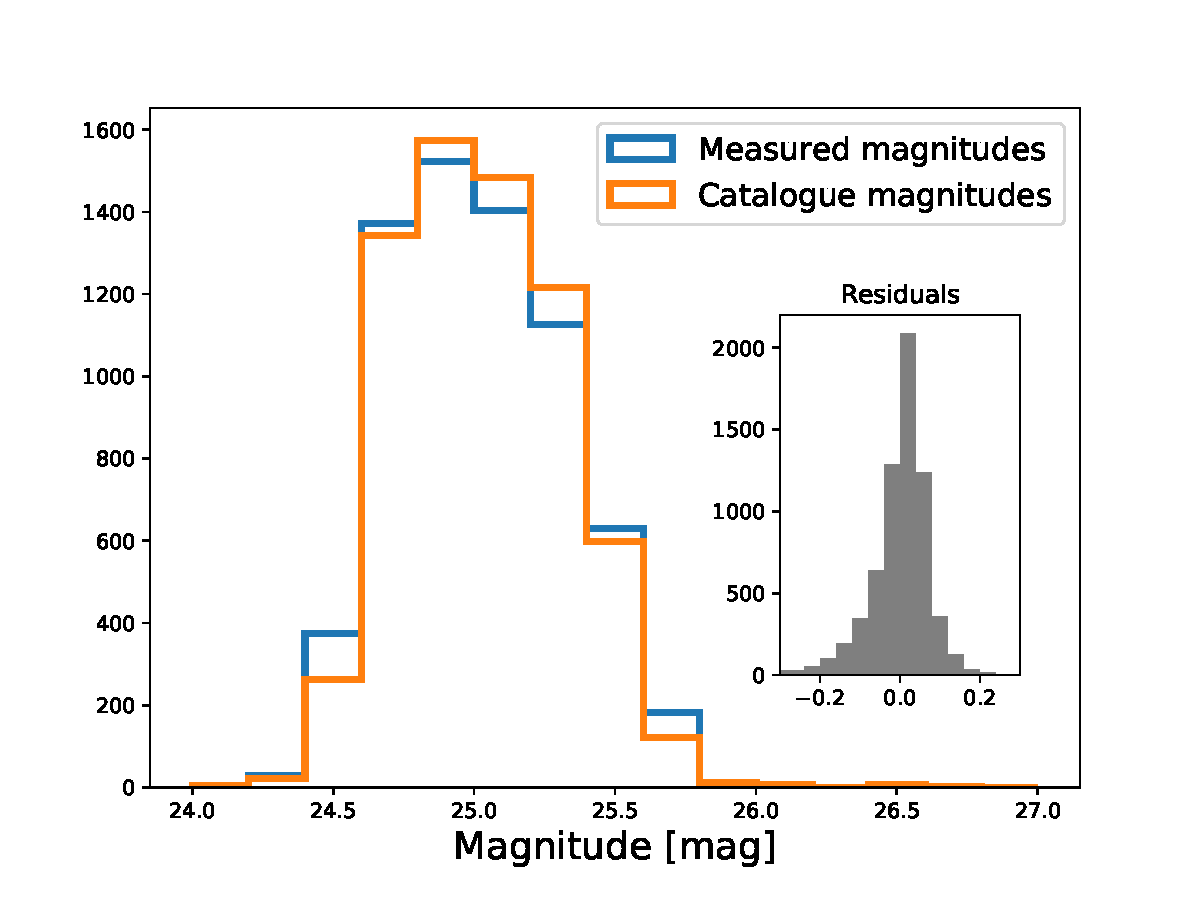
\includegraphics[trim={0.5cm 0 2cm 1.8cm},clip,width=0.45\textwidth]{Code/Saved_Figures/Mag_hist.pdf}
    \caption{The distribution of magnitudes pertaining to objects in the COSMOS field. In blue, the magnitude measurements found by running SEP is plotted. In orange the 2'' magnitudes reported in the COSMOS 2015 catalogue are displayed. In grey a residual plot is shown, mapping the difference between the measured and reported magnitude for each object.}
    \label{mag_hist}  
\end{wrapfigure}

Utilising the software IRACCLEAN presented in \cite{Hsieh_2012_IRACCLEAN}, the sources can be modelled to produce a residual map. The centroids from the SEP algorithm and the total flux found from fixed aperture photometry is used to create point source models of the sources. The point source model is an approximation, since the light profiles of the galaxies might differ from a perfect point source. However, due to the low resolution of the IRAC image, as a result of its peculiarly large point spread function (PSF) that is much bigger than the size of the galaxies modelled, the approximation is deemed reasonable. \textcolor{red}{I should probably make it clear that I didnt actually do this but refer to the author - Iary. Also convolving with PSF?}. \\ \\
There are, however, some limitations to aperture photometry and the residual map it produces. All sources in the image are modelled individually with a point source model, where the flux is a free parameter that rescales the profile to fit the source. The flux used is the total flux within a fixed aperture, hence the aperture size is an assumption we enforce on all sources, although an adaptive aperture may have been more appropriate. Typically this is not a problem as long as the aperture size is relatively large, including all flux intrinsic to the source, and the surrounding is background which values are centred around zero. The problem arises when there is a  blended pair of galaxies, and the intrinsic flux cannot be properly estimated or divided between the sources \textcolor{red}{consider moving this to the discussion}. To address the drawbacks of aperture photometry, we explore a different approach of creating a residual image. An alternative to aperture photometry is model-based photometry, a method from which the Farmer tool is developed. \\

The Farmer tool \cite{Weaver_2020}, like the previous method, also starts out with a source detection algorithm (SEP) reporting the centroids of each source detected. Next it identifies particularly crowded regions where there are multiple objects nearby each other that could present overlapping flux. Contrary to the previous methods, these sources are modelled simultaneously. Furthermore this method does not require enforcing a fixed aperture size. Instead the total flux is determined by fitting an intrinsic light profile to the source, and integrating the area below the surface. The Farmer tool fits a source to one of 5 models. Common for all of them is that they are parametrized using the centroid position of the source as a fixed parameter and the total flux as a free parameter. The models are:
\begin{enumerate}
    \item \textbf{Point Source} models are taken directly from the point spread function (PSF) used. It is similar to the method applied when using aperture photometry.
    \item \textbf{Simple Galaxy} models are circular symmetric, exponential light profile with a fixed 0.45’’ effective radius.
    \item \textbf{Exponential Galaxy} models are exponential light profiles. In addition to the common parameters these are parametrised also by effective radius, axis ratio and position angle.
    \item \textbf{DeVaucouleur Galaxy} models are de Vaucouleurs light profiles. These models require similar parameters as the exponential galaxy model.
    \item \textbf{Composite Galaxy} models are combines a Exponential Galaxy profile with a DeVaucouleur Galaxy profile. The profiles are concentric, and the model, like the others, is therefor only parametrised by one pair of centroids coordinates. Each component is parametrised by the free parameters described in the two previous models. In addition there is a “fraction of total flux” parameter that distributes the flux between the two components.
\end{enumerate}


Except for the Point Source model, they can all be described analytically by changing the parameter $n$ in a 2d Sérsic profile, which is given by \footnote{\textcolor{blue}{better reference perhaps}\url{http://ned.ipac.caltech.edu/level5/March05/Graham/Graham2.html}} eq. \ref{sersic},
\begin{equation}
   I(R) = I_e \cdot \exp \left(-b_n \cdot \left( \left( \frac{R}{R_e} \right)^{\frac{1}{n}} - 1\right) \right)
   \label{sersic}
\end{equation}
where $I_e$ is the intensity at the effective radius $R_e$ that encloses half of the total light from the model. The constant $b_n$ is defined from $n$, to make sure the total luminosity is obtained when integrating the profile. Since they are all analytical, they can easily be integrated to obtain the total flux. The real challenge lies in choosing the right model and obtaining a converging fit. The Farmer tool includes a decision tree for selecting the most appropriate model type to fit a given source with. The models are tested in the order they are described above (1 to 5), and the quality of their residuals are ranked, so the best model is chosen. When the most appropriate model type is selected for all sources, optimisation of the free parameters is performed as the final step, so that the parameters chosen for one object will not directly affect the parameters of nearby objects. \textcolor{red}{Next sentence might also be more suited for the discussion} While this method does improve on some of the drawbacks from aperture photometry, it is next to impossible to make all model fittings converge. There are a few possible reasons for the failure to converge. Sometimes a bright source is simply not well described by a smooth profile. It could also be due to a very blended pair that was not successfully separated in the detection, and thus not described correctly by a single light profile. \\
With this process, the Farmer tool can provide us with the parameters needed for creating intrinsic light profiles of the sources detected in the image. The models describe how we expect the light to look intrinsically, but when the light is observed through a telescope it is warped due to the way the imaging system responds to a point source. A point spread function (PSF) maps how a point-like object will appear in the image you are working with. Therefore, to create a residual image we need to model the objects as they would appear in the image. We obtain the final models from a convolution of the intrinsic light profiles with the PSF of the image. The residual map is then produced by subtracting the convoluted models from the telescope image, carefully placing the models right according to the detected centroid coordinates.

For the next part of the project we need a catalogue containing the coordinates and total flux of objects detected in the residual image. For this purpose we use SEP source detection and aperture photometry to estimate the total flux. This catalogue will likely contain different objects of various level of interest: spurious objects, left-over flux from subtracted sources due to imperfections in the residual image, and hopefully there will be some dropout galaxies.

\subsection{Classification with Semi-supervised Machine Learning}
In this thesis we develop a semi-automated method of selecting NIR-dropout galaxies based on t-distributed Stochastic Neighbour Embedding (t-SNE) \cite{Maaten_2008_tSNE} and k Nearest Neighbour (kNN) voting. This method uses as input: 4 telescope images \textcolor{red}{telescope cutouts/ images with the galaxy centred/poststamps/vignettes - find the right description} of each galaxy in the sample, from respectively the $H$, $Ks$, $ch1$ and $ch2$ bands. The method is semi-supervised, and hence will need some parameter tuning along the way and some labels. With this, the technique will predict whether each galaxy in the sample is a dropout or not.

\subsubsection{Dimensionality Reduction with t-SNE}
\textcolor{blue}{if possible include the example of handwritten digits to show how it works}
As mentioned, the input that the method is given for each object in the sample is four small telescope images centred at the object in question. We use cutouts of the size $21\!\times\!21$ pixels, meaning that we in total will have $21\times21\times4=1764$ features for each object in the sample. Inherently, this is a very high-dimensional classification problem, and it is particularly difficult to produce meaningful predictions from, when the learning is unsupervised. A way to simplify the problem is embedding the high-dimensional data in a 2-d representation. There are many approaches to obtaining such an embedding, but for our purposes we will adopt the method of t-SNE, which has gained a lot of popularity since its release in 2008 \textcolor{blue}{quantify this more how many paper used it in astrophysics etc}. A recent NBI paper \cite{Steinhardt_2020} proposed this novel technique for classification of galaxies from photometric data, which has inspired the approach applied here. In particular they used t-SNE to classify quiescent galaxies from their spectral energy distributions (SEDs). \\

t-SNE takes a set of high dimensional vectors, in this case the pixels originating from four different images, and computes the euclidean distance between each vector. From this it calculates a probability that two vectors should be considered neighbours. This probability considers the user-specified hyper parameter \textit{perplexity}, which determines the sizes of the neighbourhoods based on the density of the data in the respective regions. The hyper parameter can effectively be understood as a estimate for the number of neighbours that should be considered similar. Values between 1 and 50 are suggested by the author to be the most effective/appropriate \cite{Maaten_2008_tSNE}. A low perplexity emphasizes local structure in the embedding, while a high perplexity will preserve more of the global structure of the samples. A universally good perplexity value cannot be determined, but should be selected manually for each data set. This is because the density of the objects varies depending on the sample size, and thus the number of optimal neighbours will vary. The perplexity is chosen, in this thesis, by performing the t-SNE embedding for various perplexities and determining which structure is best suited for the purpose of classifying dropouts. \\
t-SNE is stochastic in its nature, and will thus compute different embeddings for the same data set unless the same random seed is specified every time. To be able to reproduce our results, this was therefore implemented. Its stochastic nature lies in the fact that it will try out different configurations for the embedding and evaluate the probabilities, which it will try to improve in the next iteration. Due to the huge dimension of the data, this makes the process much faster, but also means that the embedding is not reversible, and new objects cannot be added individually to the embedding space. All data thus has to be given to the algortihm at once. We can specify the maximum number of iterations for the procedure, and the code/algorithm will output the number of iterations it actually used to produce the embedding. This means we can also use the number of iterations as a tool for choosing the right perplexity. If the number of iterations is smaller than the maximum number of iterations, this means the embedding has converged in the sense that it could not find a better configuration for the embedding during the next 300 iterations. \\
Since the t-SNE algortithm is a form of unsupervised machine learning, the embedding map will be produced without any direct knowledge of what a dropout galaxy looks like. It will however place objects it considers similar close to each other, even though the algorithm is unaware that the features are pixels from a series of telescope images. This is also one of the reasons t-SNE is so popular: the flexibility in its applications makes it a very powerful tool\textcolor{red}{perhaps mentions of where it is also used other than astronomy}. For our purpose it is useful because the photometric information that is stored in the difference in the image cutouts is an indicator of dropout galaxies.

\subsubsection{The Use of Tracers in the Embedding}
So far the classification process has been completely unsupervised, but now that a 2-d representation of the sample is obtained, we need to understand in which region  dropout galaxies are located.  By selecting "tracers" in our sample, we can map where they are placed in the embedding by the t-SNE algorithm. If the tracers cluster well, this is a good indication of a promising region for finding NIR-dropouts. \\

Tracers is how we will refer to the objects we have determined to be reliable candidates of NIR-dropouts. These are selected based on a visual inspection of the objects in the four bands. We look for objects that are visible in IRAC $ch1$ and $ch2$, and which do not appear in the NIR bands $H$ and $Ks$. Since the objects we look for are similar to those found in \cite{Alcalde_Pampliega_2019} and \cite{Wang_2019}, we can also use these as a reference. An example of which objects we would classify as a tracer is displayed in fig. \ref{tracer_example}. Having identified a sub sample of tracers, we can use these both for producing predictions and for validating our results.
\begin{wrapfigure}{r}{0.4\textwidth}
    \centering %left, lower, right, upper
    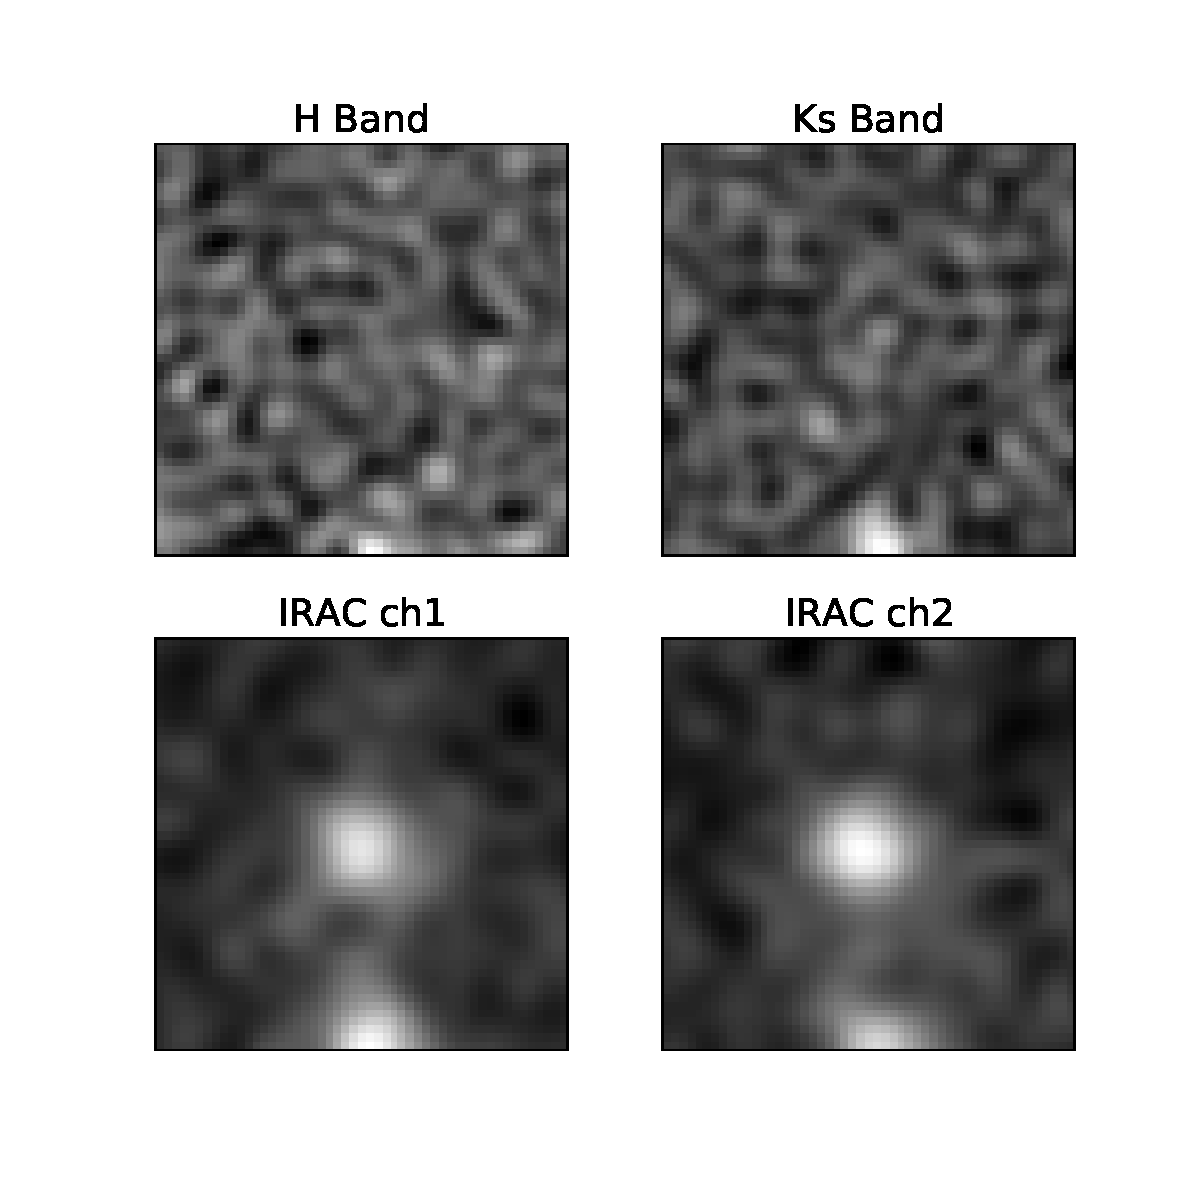
\includegraphics[trim={1cm 2.5cm 2cm 1.5cm},clip,width=0.38\textwidth]{Code/Saved_Figures/good_example.pdf}
    \caption{An example of a tracer for NIR-dropouts. The object is clearly visible in the IRAC bands, while it drops out in the NIR bands.}
    \label{tracer_example}  
\end{wrapfigure}
\textcolor{blue}{missing: we also selected bad candidates}

\subsubsection{Classification with kNN voting}
Now that we have an embedding that is more easily visualised and interpreted and we have tracers indicating the interesting regions \textcolor{blue}{and bad regions}, we can construct the semi-supervised algorithm used to produce predictions on the sample. An object can either be classified as a NIR-dropout or a non NIR-dropout galaxy. The method takes basis in the principle of k nearest neighbours (kNN) and voting. \\
The code performing the classification is divided into the following modules:
\begin{enumerate}
    \item First, the distances between an unknown object and all tracers are computed, from which the k nearest tracers are selected (a range of values $1<k<10000$ will be tested).
    \item The votes of the k neighbours are then collected. A neighbour that has been previously labelled as good tracer  will vote for a NIR dropout prediction, while a bad tracer will vote against.
    \item It is checked if the fraction of positive votes  is above the threshold $f_{min}$, which defines the minimum fraction  required for predicting a dropout. In the following we will experiment different values of $f_{min}$, from X to Y\%. 
    \item On behalf of the above, the predictions are computed.
\end{enumerate}
An alternate strategy would be collecting votes from all the neighbours within a fixed radius in the 2-d space. 
The choice of using nearest neighbours instead of this other option  is based on two considerations. First of all the two dimensions of the t-SNE embedding are arbitrary, thus defining a physically meaningful radius is challenging. Furthermore, the embedding represents an approximation of the higher dimensional distribution of objects, and therefore we cannot be certain that a euclidean distance in one region of the embedding is consistent with the distance measured in another region. Assuming a uniform density of objects in the embedding, letting the k nearest neighbours would in turn provide a more consistent voting. By introducing the threshold $f_{min}$, we are able to modify our selection of NIR dropouts based on the desired balance of quality and quantity. One can then select a parameter of $f_{min}$ that identifies fewer, more robust dropout candidates or be less conservative but... \textcolor{red}{Maybe elaborate on the purity measure shown in the results}.
\textcolor{red}{Should I include a desciption of what a ROC curve is? I am familiar with the concept from many courses so I dont feel it is necessary, but perhaps the censor is not familiar with it? not sure}

\section{Results}

\subsection{Residual Map}
\begin{itemize}
    \item Show one of each of the type of models used to make the residual map. Possibly include the entire image in appendix or link to a fits file containing the image.
    \item Stats from the modelling. How many of each type, which is the most common etc. How many models failed.
    \item Mention the masks (maybe in method instead) covering bright spots that are not included in the cosmos catalogue since they were corrupt.
    \item Think about running the source detection on this image as was the plan and provide some stats of the result.
    \item Mention that we ended up using the residual image Iary made weighing the channel 1 and 2 images of IRAC. Explain quickly how this was made, and why we believe it to be more robust than the residual map I myself created. Elaborate on this in the discussion. The FARMER catalogue is still not finished developed
\end{itemize} 

\begin{wrapfigure}{r}{0.4\textwidth}
    \centering %left, lower, right, upper
    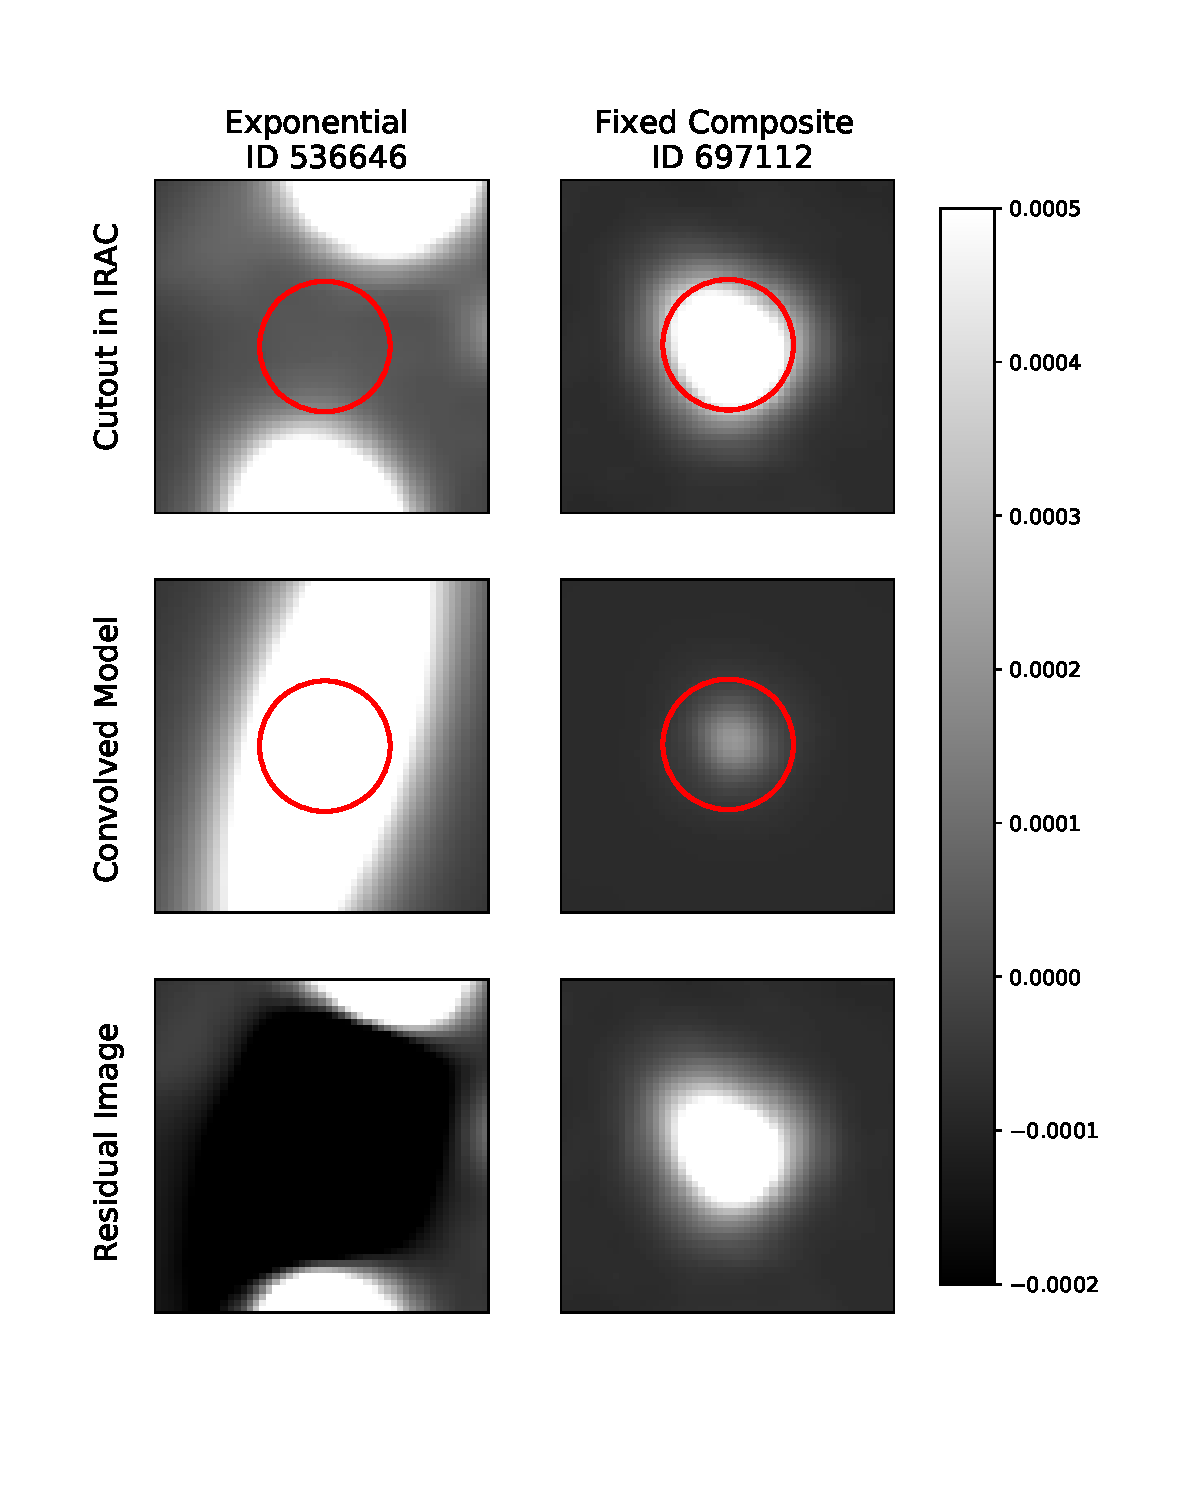
\includegraphics[trim={1cm 2.5cm 2cm 1.5cm},clip,width=0.38\textwidth]{Code/Saved_Figures/BAD_model_cutouts.pdf}
    \caption{hi}
    \label{BAD_Model_cutouts}  
\end{wrapfigure}

\begin{figure}[h!]
    \centering
    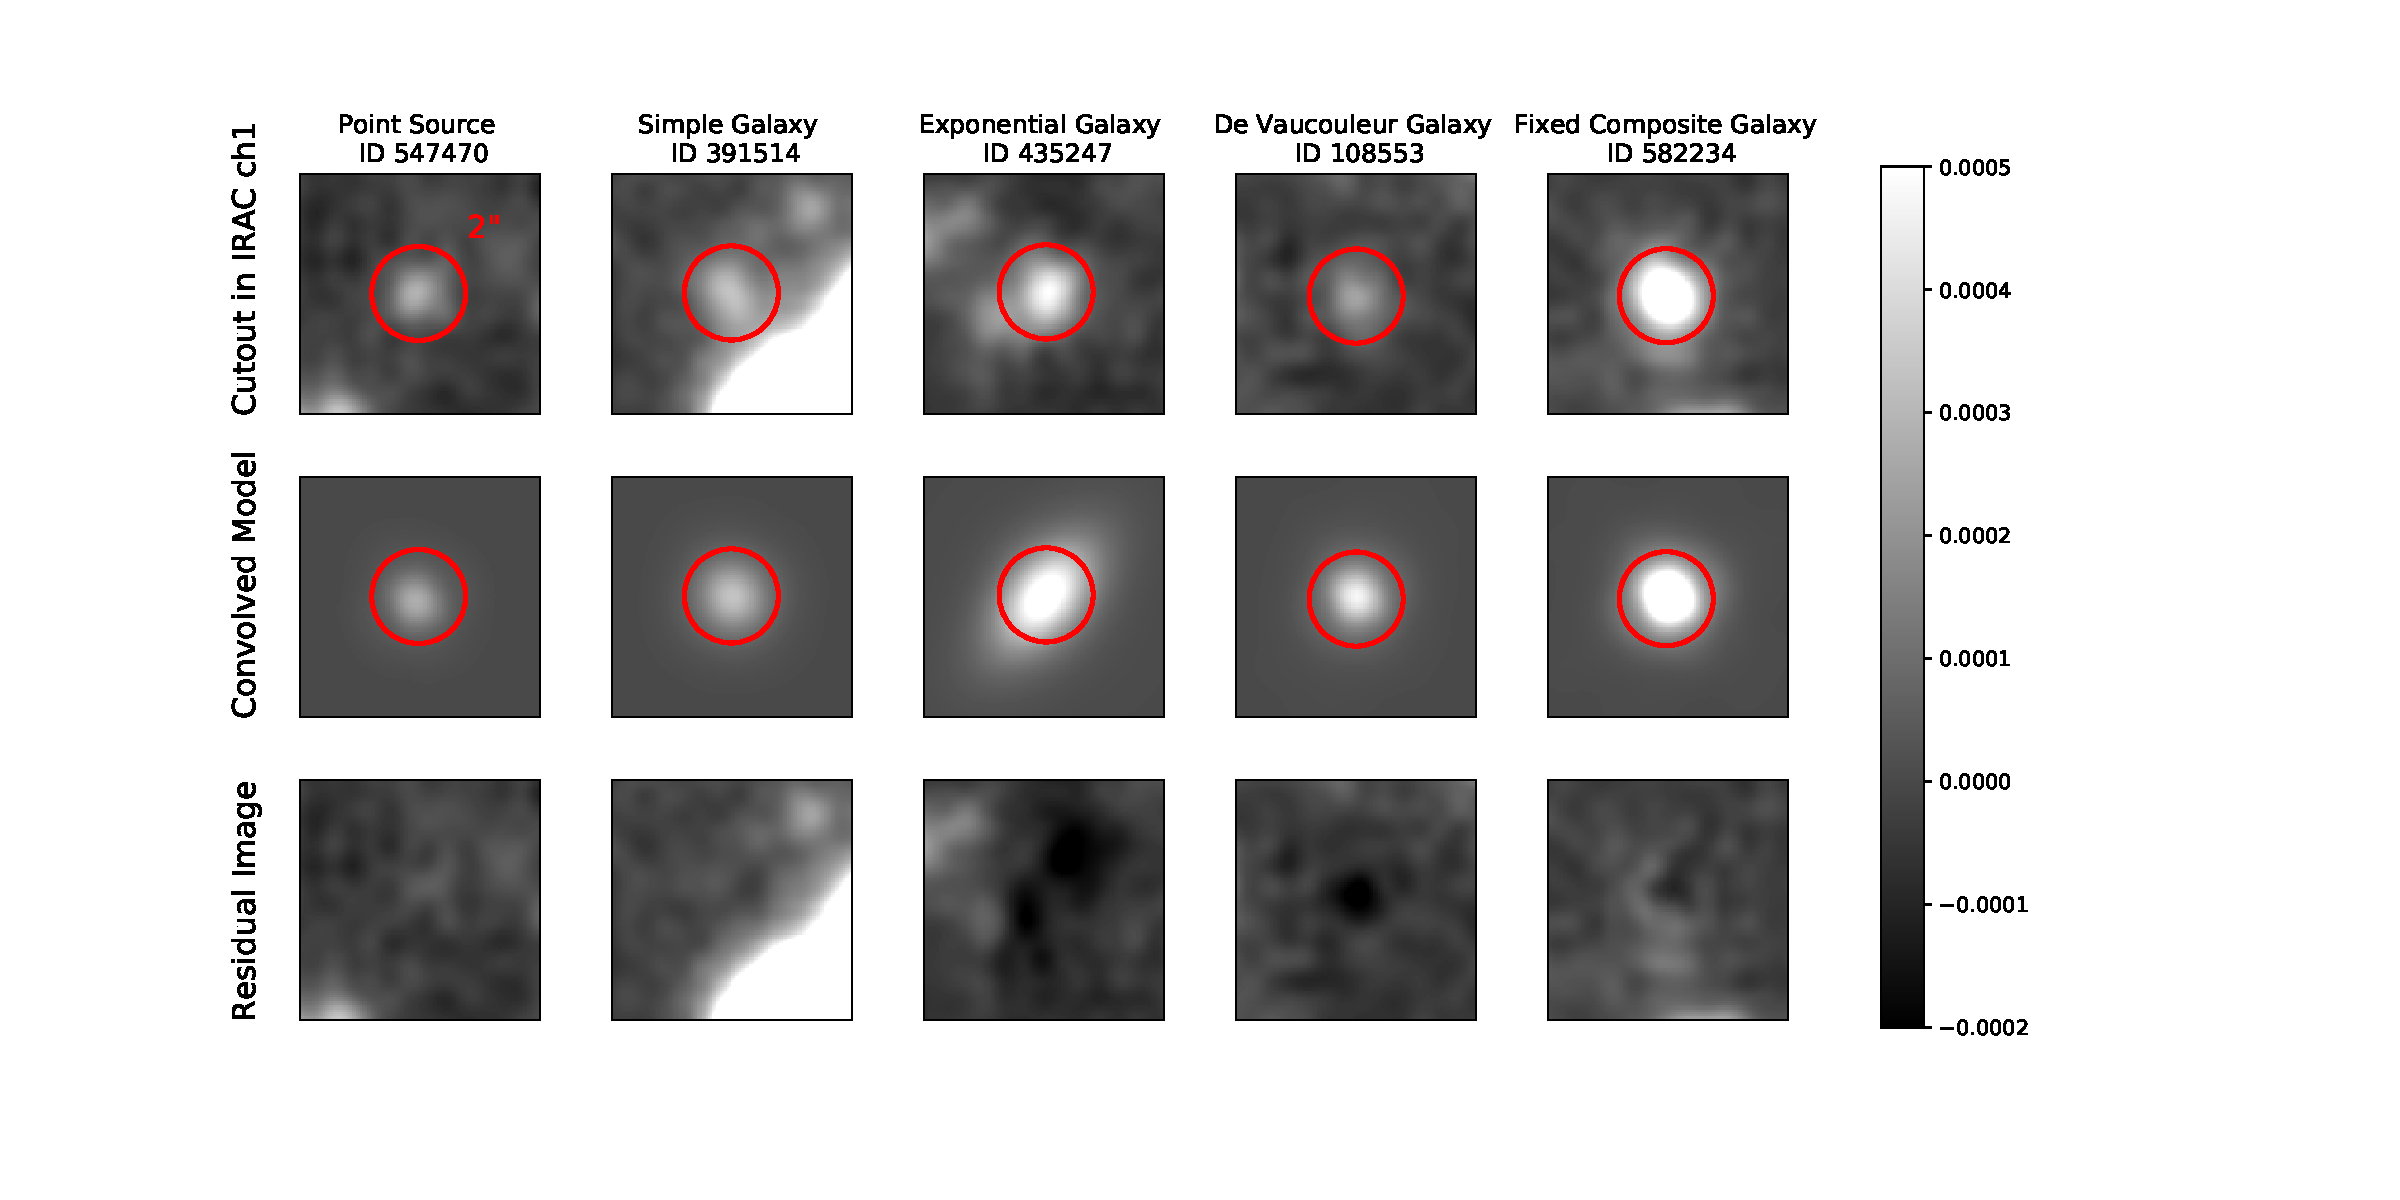
\includegraphics[trim={3cm 2.5cm 5cm 1.5cm},clip,scale=0.5]{Code/Saved_Figures/Model_cutouts.pdf}
    \caption{hi}
    \label{Model_cutouts}
\end{figure}

\subsection{Dimensionality Reduction}
\begin{itemize}
    \item t-SNE embedding plot with varying perplexities and colors (blue-red) colormapped. Describe the corrupted flux marked in another color. Include the most interesting one - "k-c1" here, "h-k" and "ch1-ch2" can be added in the appendix.
    \item Describe why that perplexity is chosen. Describe the color distribution. There are two outliers or so that fall distant from the main cluster, quickly look to these and describe why we omit them from the analysis.
    \item Describe our use of tracers - how many good ones were there and a few stats.
    \item Show the results on the chosen perplexity. Main plot = t-SNE embedding where the matched objects, good candidates and fluxes above some threshold is colormapped. This allows us to mark three regions, and we display cutouts from at least one object in each region as subplots around the embedding plot.
\end{itemize}

\begin{figure}[h!]
    \centering %left, lower, right, upper
    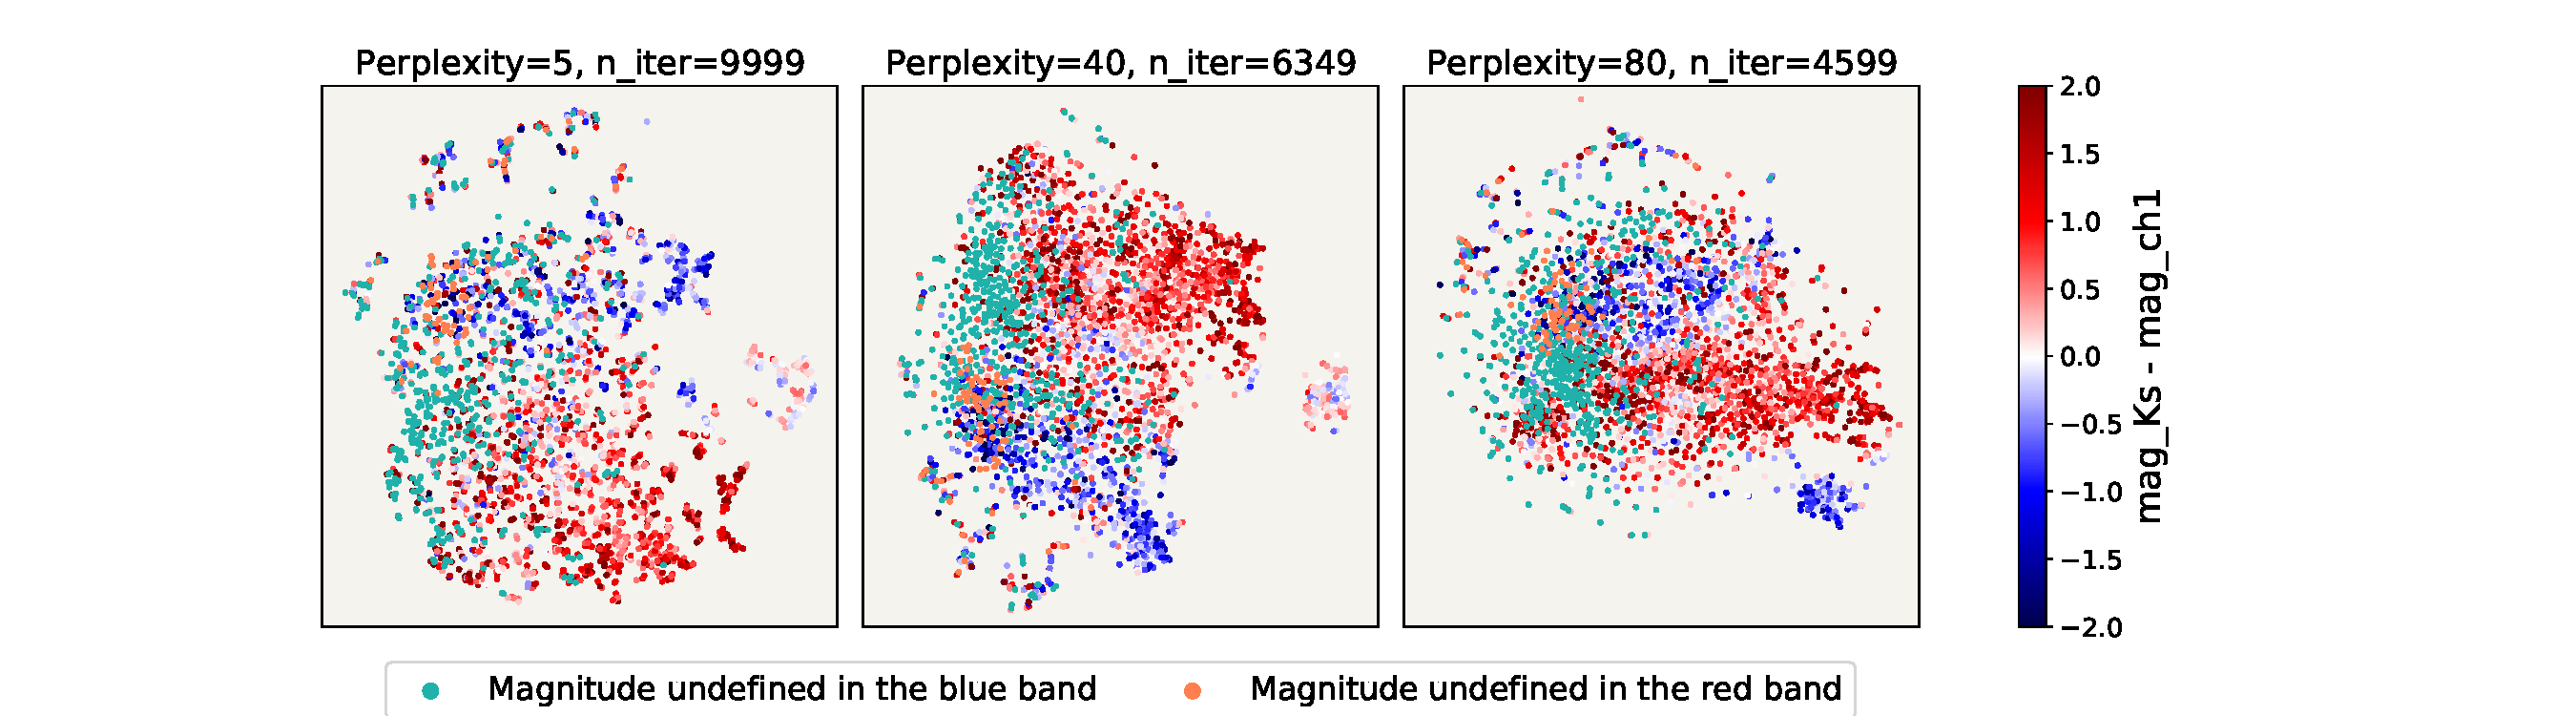
\includegraphics[trim={5cm 0cm 5cm 0.5cm},clip,width=\textwidth]{Code/Saved_Figures/peplex_Ks_ch1_SMALL.pdf}
    \caption{hi}
    \label{SMALL_embeddding_ks_ch1}
\end{figure}

\begin{figure}[h!]
    \centering %left, lower, right, upper
    \includegraphics[trim={0cm 0cm 0cm 0cm},clip,width=\textwidth]{Code/Saved_Figures/}
    \caption{hi}
    \label{SMALL_embeddding_ks_ch1}
\end{figure}

Perplexity 40 is chosen since the result is a nice cluster with clearly seperated blue and red galaxies (see figure \ref{SMALL_embeddding_ks_ch1}). Additionally the n-iter ended up 6349 whcih is less than max-iter of 10000, meaning that the embedding converged. Peplexity 80 and 100 also converged but the original paper \cite{Maaten_2008_tSNE} suggests choosing perplexities between 5 and 50. All perplexities tested is seen in appendix along with the color between the other bands.

\subsection{Classification / Identifying Promising Candidates}
\begin{itemize}
    \item Show the classifications on the embedding. Two subplots, one showing the embedding colores according to the labels that are known to the algorithm and one according to the predicted labels.
    \item Acompany this with a score metric. Accuracy, contamination rate and a confusion matrix are good scores to show. And write which parameters where chosen, what is k, what is fmin and so on.
    \item Produce the plot we talked about in mondays meeting similar to figure 4 in \cite{Steinhardt_2020}. A plot as a function of fmin showing contamination and the size of each population (good and bad) acompanied with a ROC curve.
    \item Include the SED plots, and show that our candidates look as we expect. Faint in H and K and more bright in ch1 and ch2.
\end{itemize}

\section{Discussion}

- What are pros and cons of the Farmer method? Is the Farmer residual image better than Iary's old one?

- Is ML really better than visual classification? pros and cons of t-SNE.

- How the COSMOS dropout galaxies look like? (eg colors, etc) 
Do they ``agree'' with previously discovered droupouts?

- A very quick discussion/speculation about how these objects fit into the "big picture" of galaxy evolution. 


\section{Conclusion}

summary.

next steps (short-term): cross-match with ALMA, X-ray, etc. SED fitting...

future perspective (long-term):  follow-up with James Webb Space Telescope.


%%%% No more document input %%%%

% Bibliography
\newpage
\addcontentsline{toc}{section}{References}
\printbibliography[title=References]


\newpage
\begin{appendices}
\pagenumbering{roman} %sidetal
\section{Source Detection in Optical and NIR bands}

\begin{figure}[h!]
    \centering
    \includegraphics[trim={5cm 3cm 5cm 3cm},clip,width=\textwidth]{Code/Saved_Figures/Source_Detection_Results.pdf}
    \caption{hi}
    \label{Source_detection}
\end{figure}

\begin{figure}[h!]
    \centering
    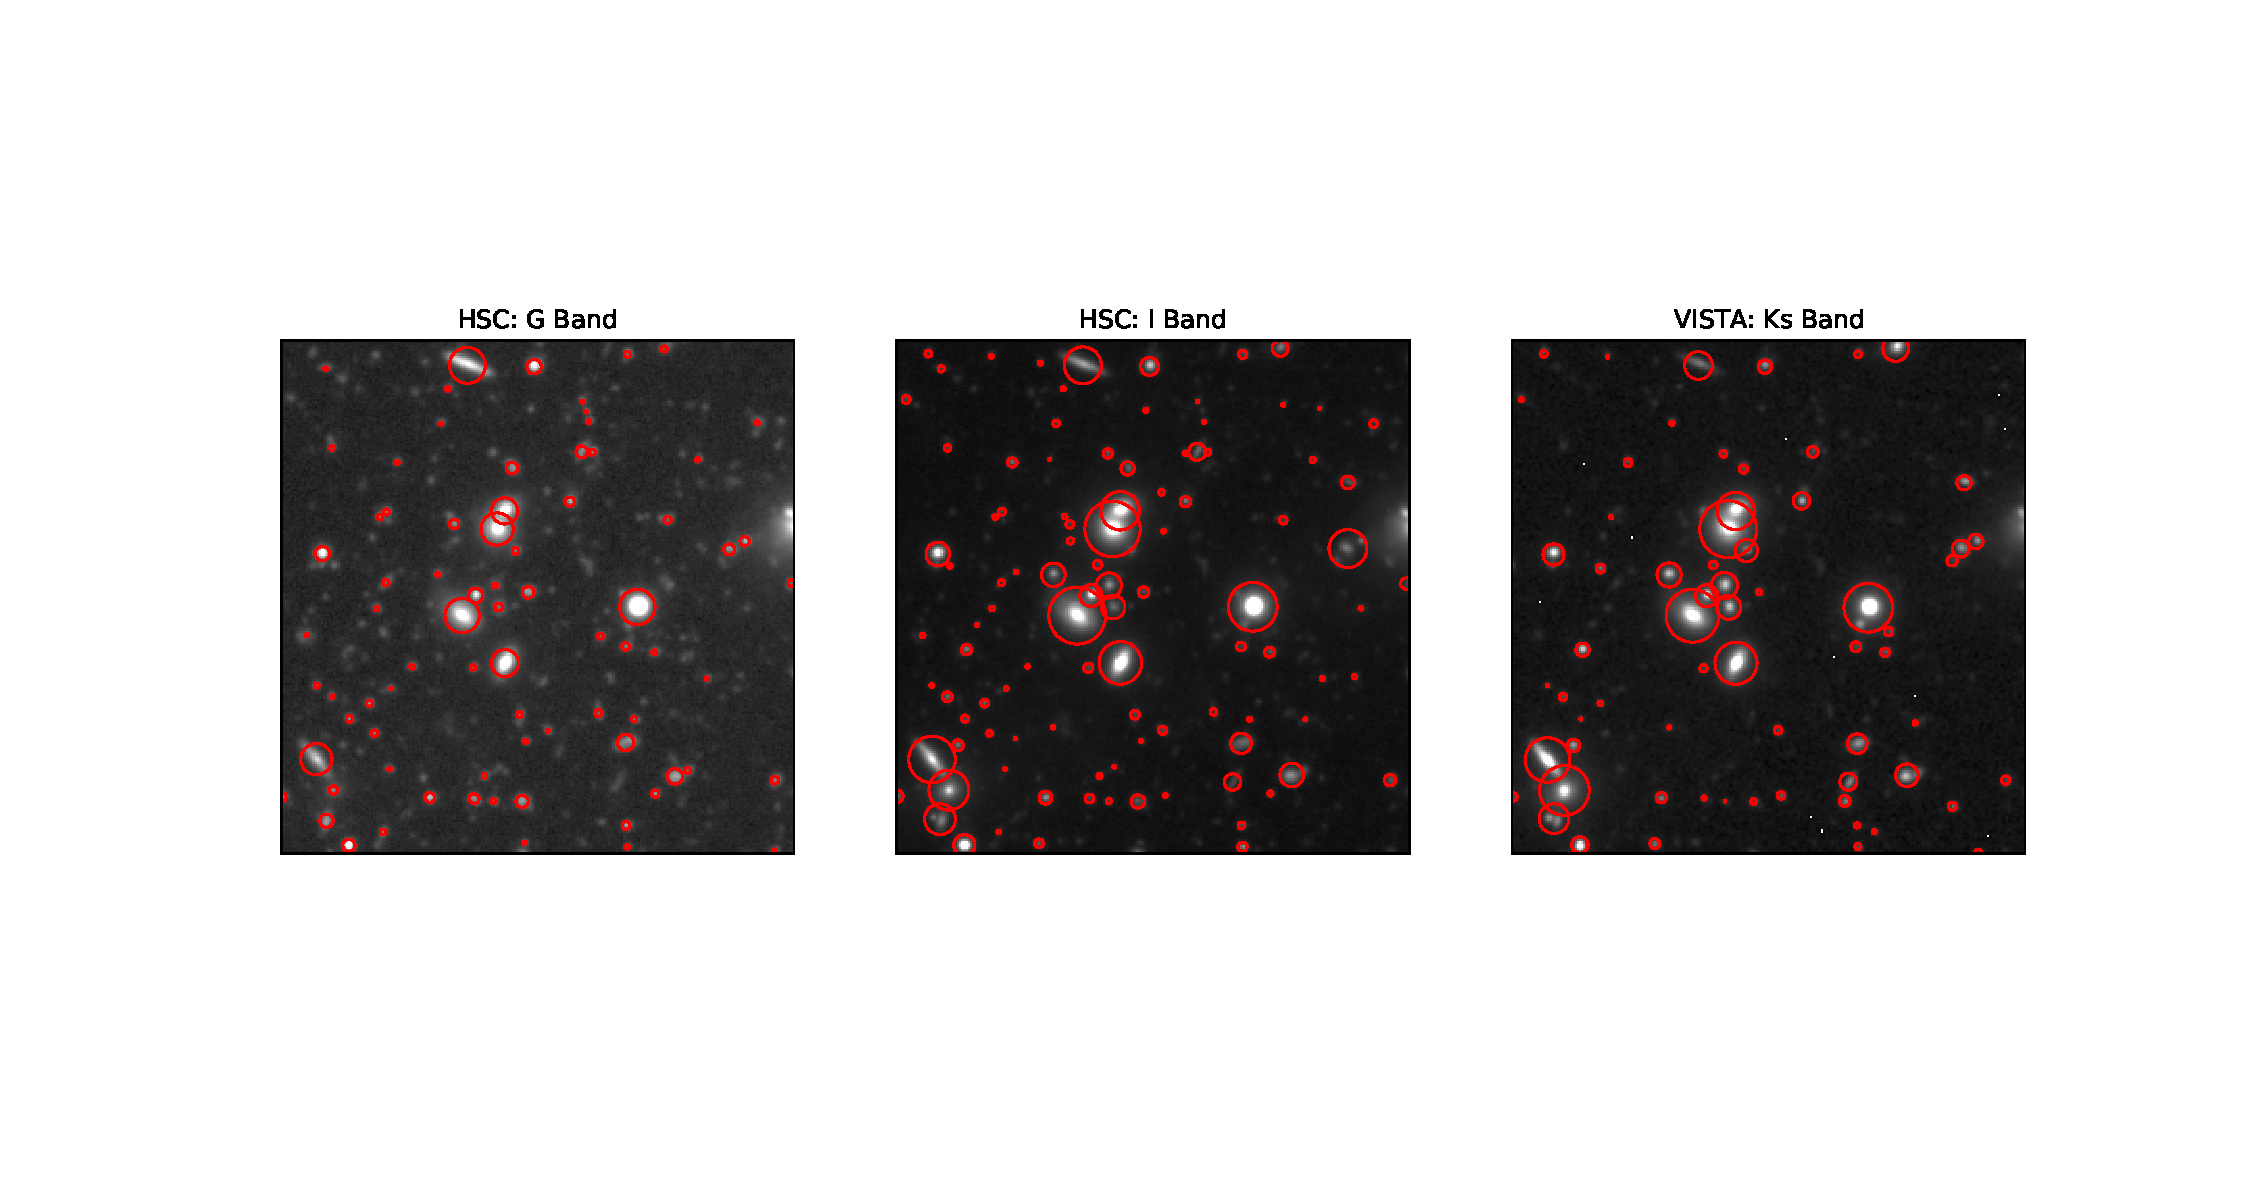
\includegraphics[trim={5cm 3cm 5cm 3cm},clip,width=\textwidth]{Code/Saved_Figures/Source_Detection_Zoom.pdf}
    \caption{hi}
    \label{Source_detection_Zoom}
\end{figure}

\newpage
\section{Residual Map}

\begin{figure}[h!]
    \centering
    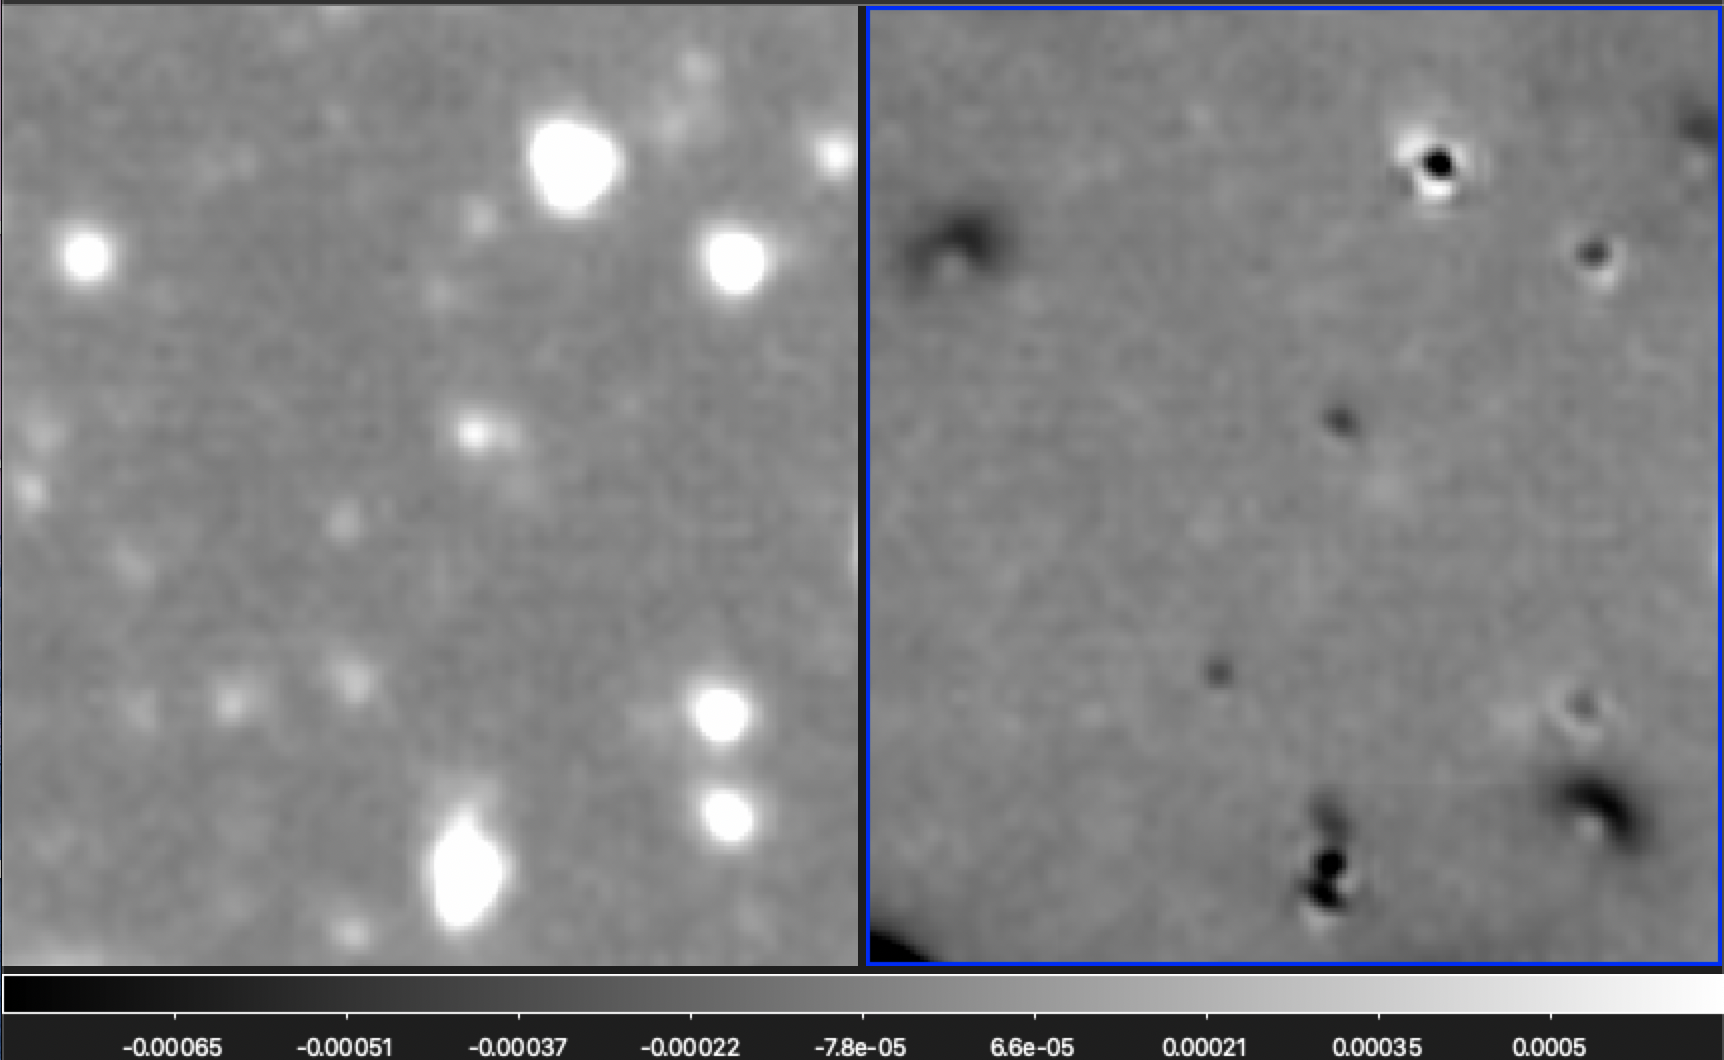
\includegraphics[scale=0.5]{Code/Saved_Figures/comparing_residual_maps}
    \caption{hi}
    \label{Comparing_residual_maps}
\end{figure}

\newpage
\section{Color Mapped t-SNE Embeddings}

\begin{figure}[h!]
    \centering
    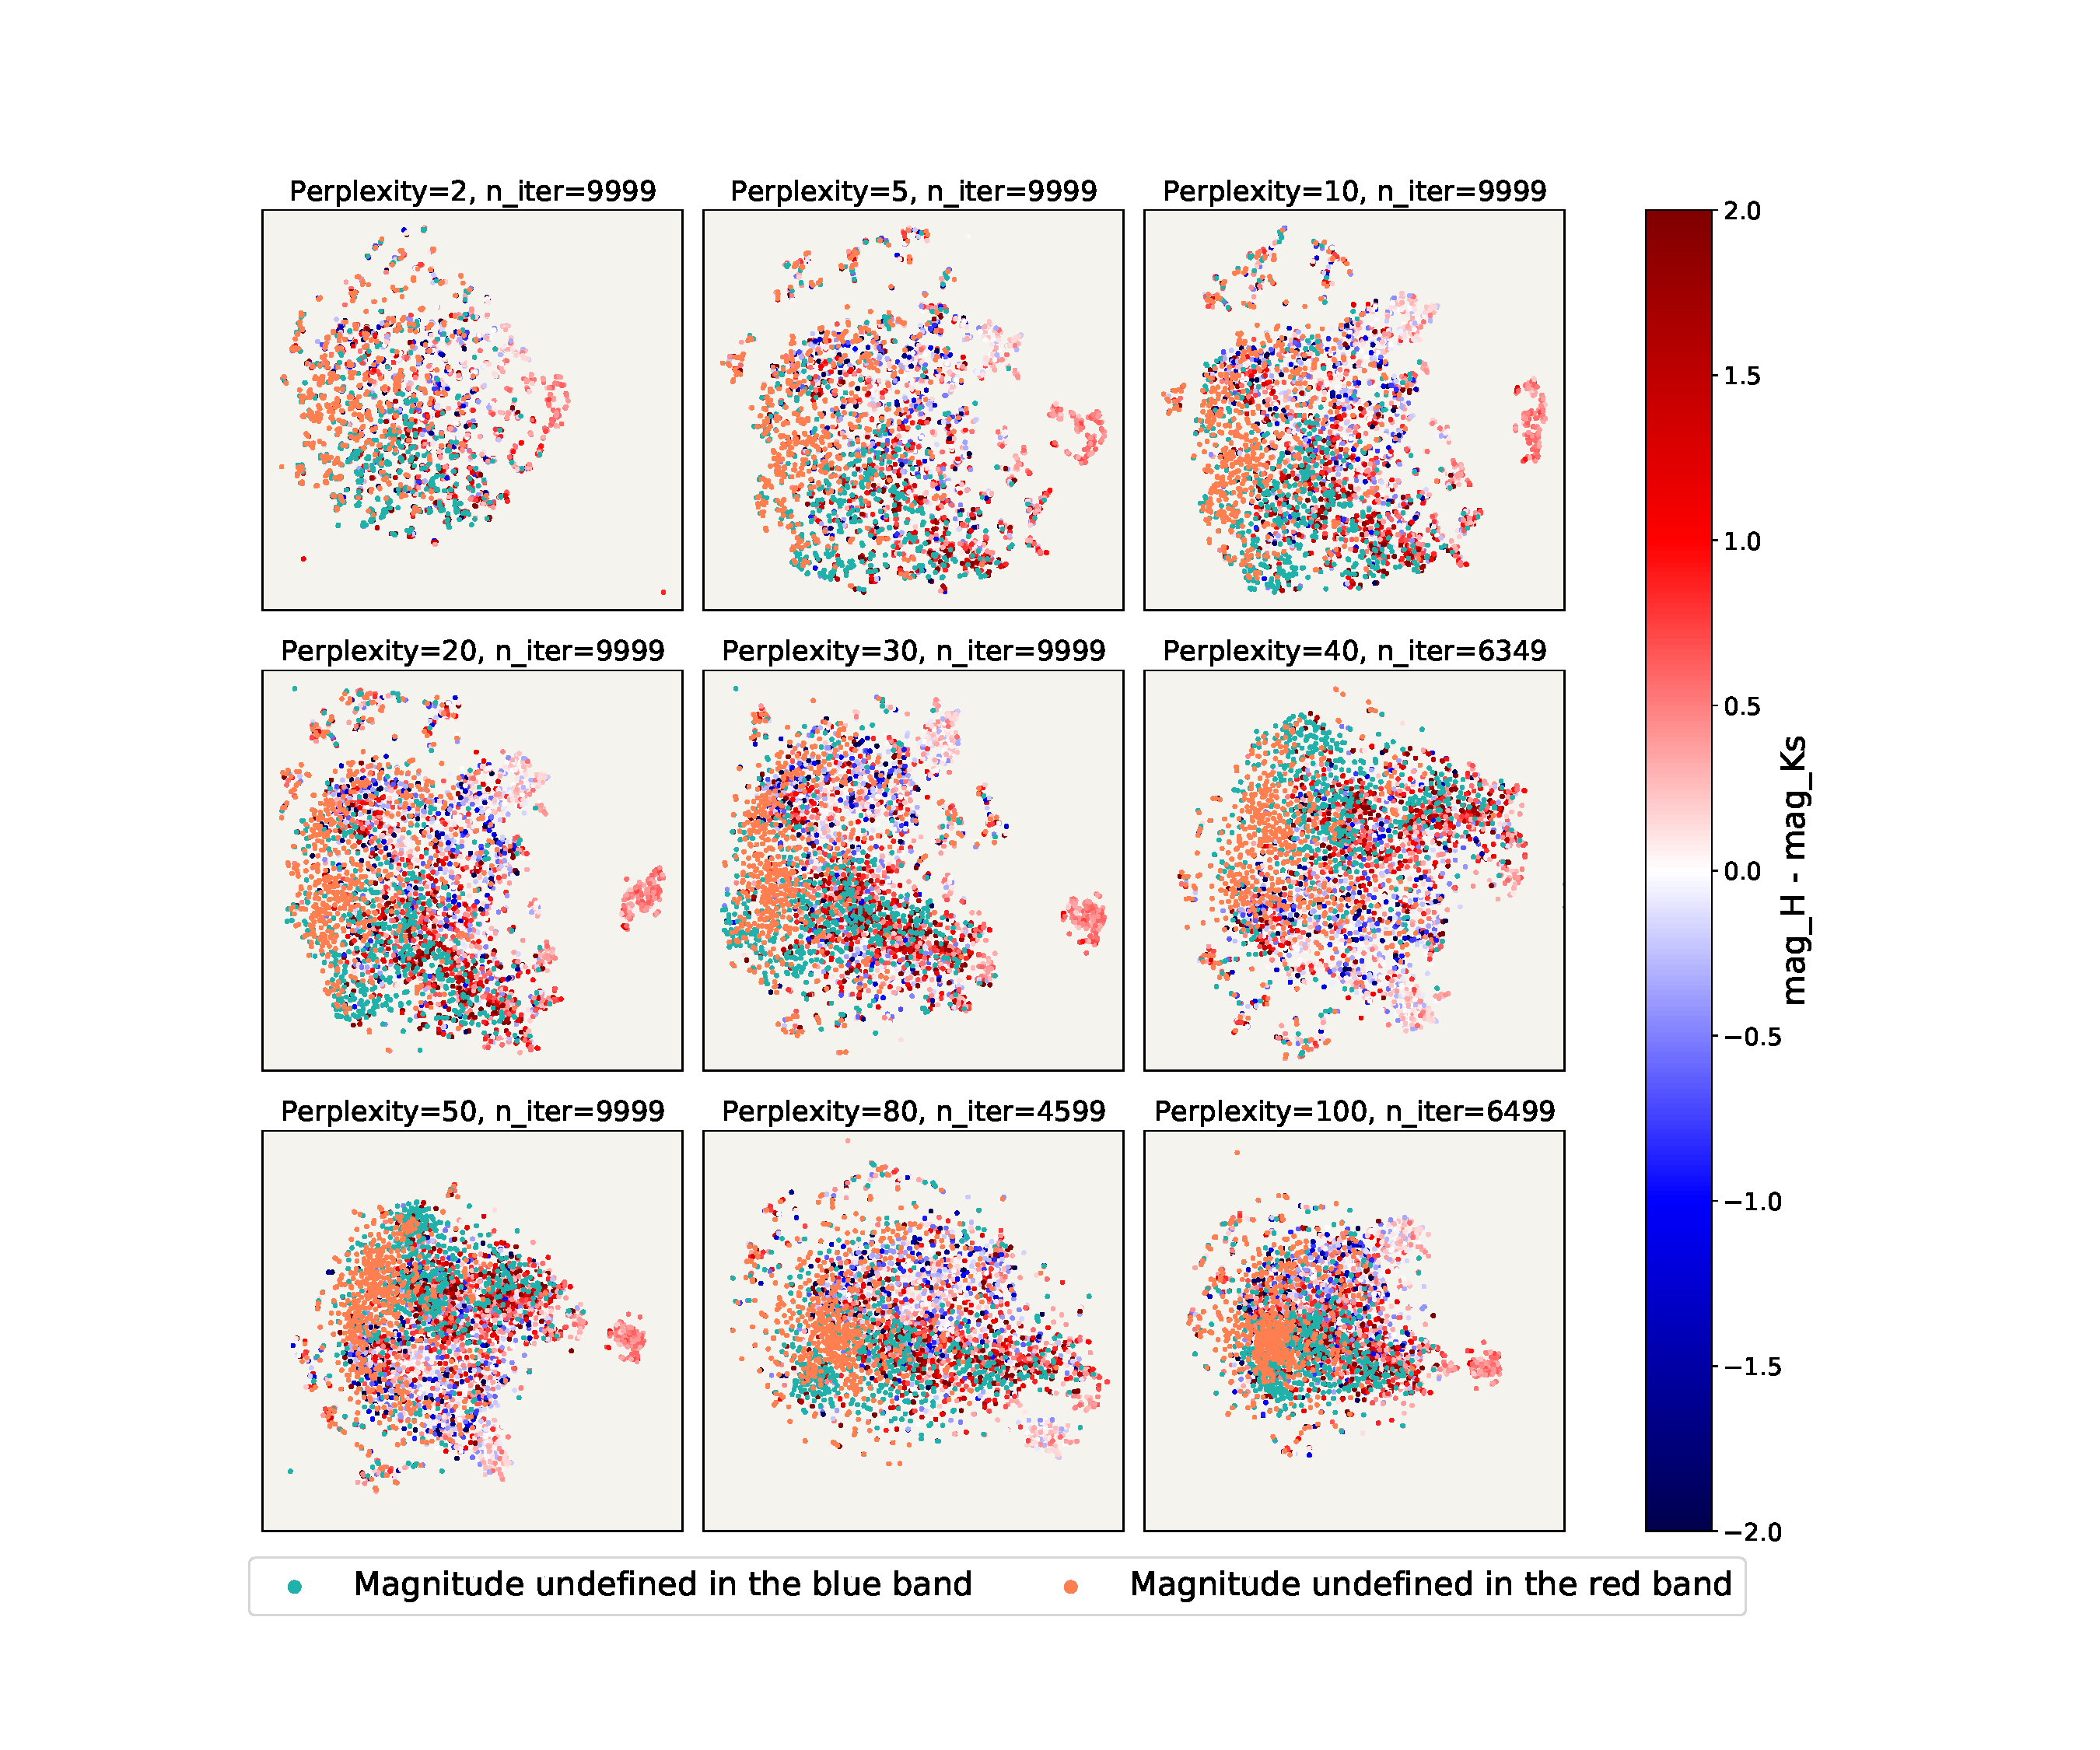
\includegraphics[trim={5cm 3cm 5cm 3cm},clip,width=\textwidth]{Code/Saved_Figures/peplex_H_Ks.pdf}
    \caption{hi}
    \label{embeddding_H_ks}
\end{figure}

\begin{figure}[h!]
    \centering
    \includegraphics[trim={5cm 3cm 5cm 3cm},clip,width=\textwidth]{Code/Saved_Figures/peplex_Ks_ch1.pdf}
    \caption{hi}
    \label{embeddding_ks_ch1}
\end{figure}

\begin{figure}[h!]
    \centering
    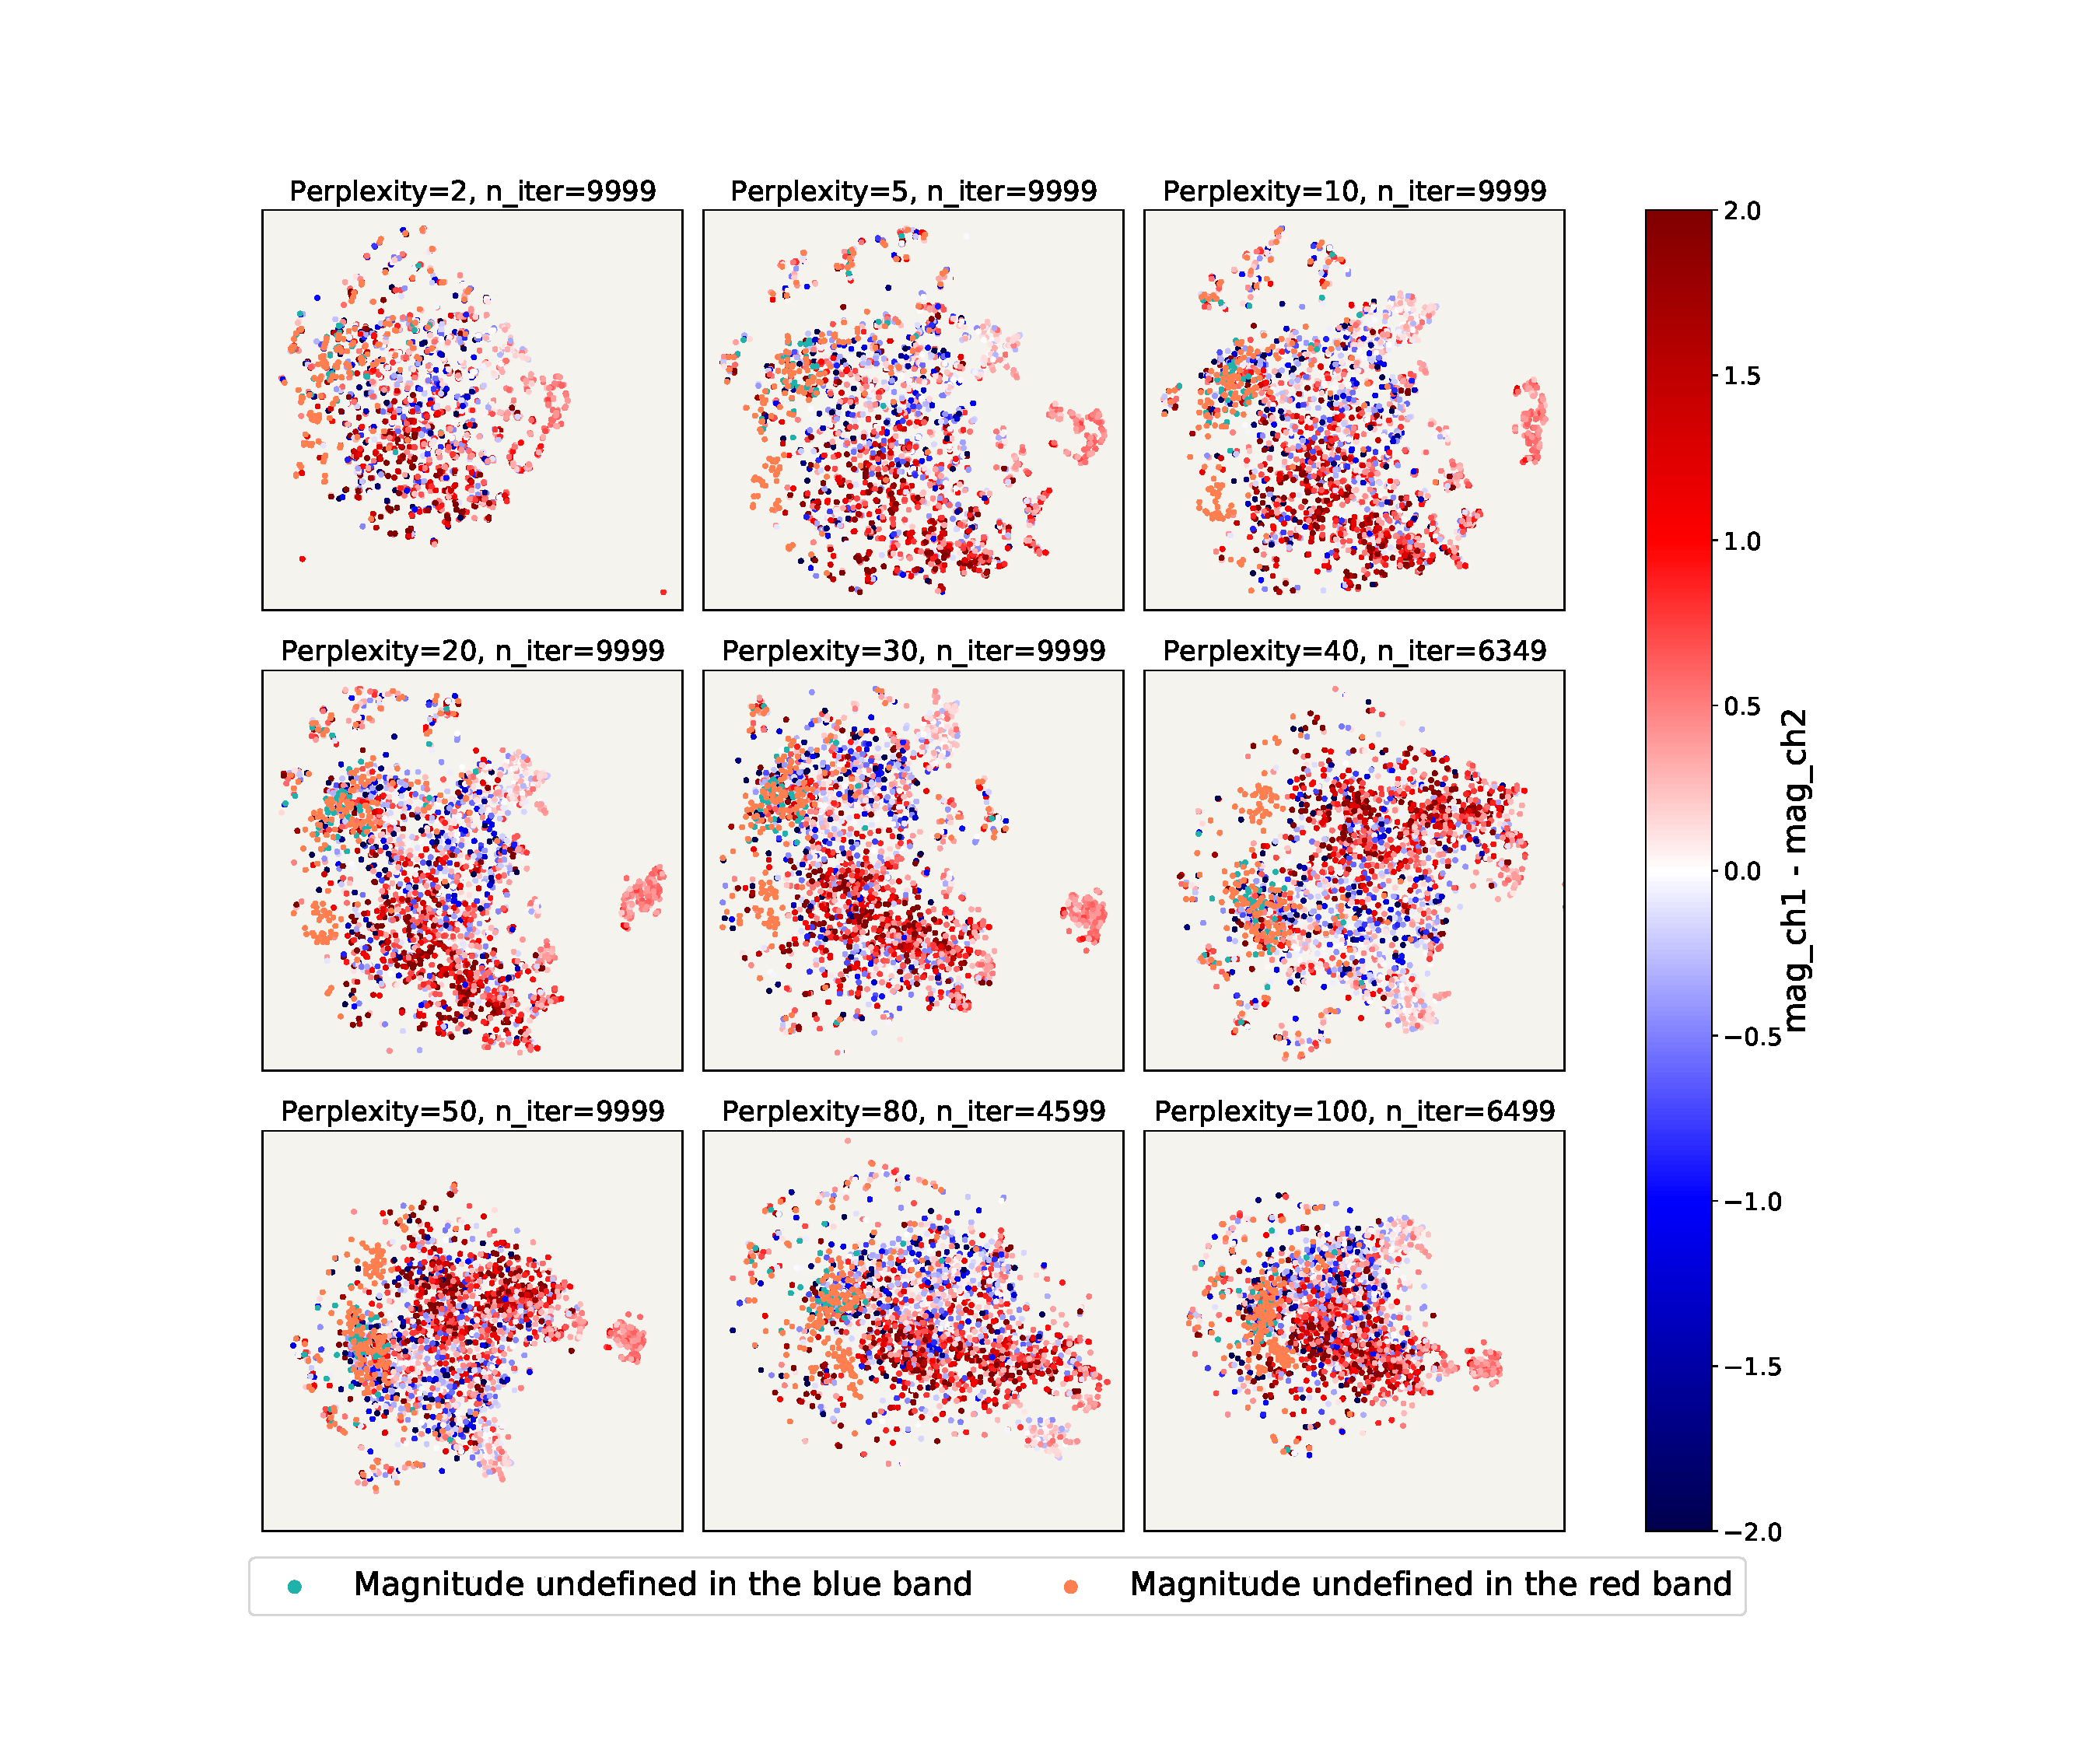
\includegraphics[trim={5cm 3cm 5cm 3cm},clip,width=\textwidth]{Code/Saved_Figures/peplex_ch1_ch2.pdf}
    \caption{hi}
    \label{embeddding_ch1_ch2}
\end{figure}
\end{appendices}


\end{document}
